% 原书印刷24–28页，PDF物理55–59页.
\subsection{分布函数}\label{sec:1.5}
对每个随机变量$X$，都关联一个称为$X$的累积分布函数的函数.
\begin{definition}\label{def:1.5.1}\index{SI0237@累积分布函数}
随机变量$X$的累积分布函数（cumulative distribution function，cdf）记为$F_X(x)$，定义为
$$F_X(x)=P_X(X\le x),\qquad\text{对所有$x$}.$$
\end{definition}

\begin{example}[抛三枚硬币]\label{ex:1.5.2}
考虑抛三枚公平硬币的试验，令$X=\text{观察到正面的次数}$.$X$的cdf为
\begin{equation}\label{eq:1.5.1}
F_X(x)=\begin{cases}
0,&-\infty<x<0,\\
\frac18,&0\le x<1,\\
\frac12,&1\le x<2,\\
\frac78,&2\le x<3,\\
1,&3\le x<\infty.
\end{cases}
\end{equation}
阶梯函数$F_X(x)$的图像见图\ref{fig:1.5.1}.从该图有几点值得注意.$F_X$对所有$x$都有定义，而不只对$\mathscr X=\{0,1,2,3\}$中的值有定义.例如，
$$F_X(2.5)=P(X\le2.5)=P(X=0,1\text{或}2)=\frac78.$$
注意，$F_X$在$x_i\in\mathscr X$处发生跳跃，且在$x_i$处的跳跃大小等于$P(X=x_i)$.又因为$X$不可能为负，所以$x<0$时$F_X(x)=0$；因为$X$必然不超过这样的值，所以$x\ge3$时$F_X(x)=1$.
\end{example}


\sourcepageanchor{56}

\begin{figure}[htbp]\centering
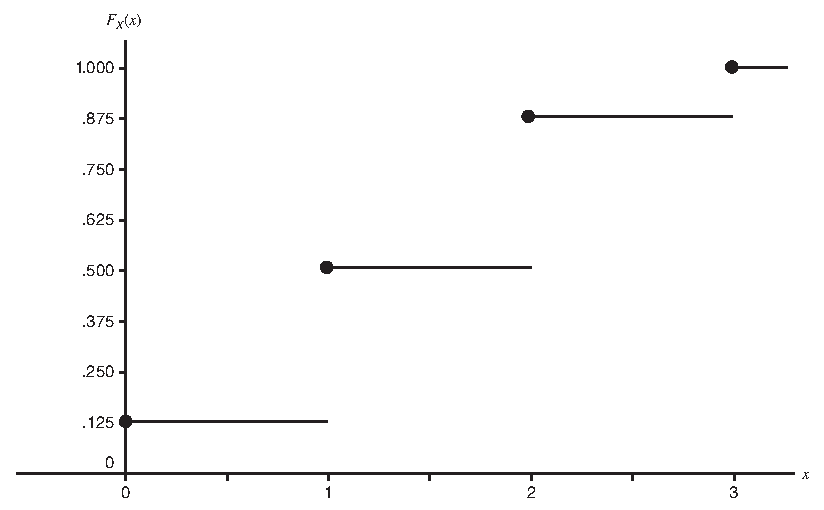
\includegraphics[width=.88\textwidth]{assets/chapter1/fig-1-5-1.pdf}
\caption{例\ref{ex:1.5.2}的cdf}\label{fig:1.5.1}
\end{figure}

从图\ref{fig:1.5.1}可以清楚地看到，$F_X$可能不连续，在某些$x$值处有跳跃.不过，由$F_X$的定义可知，在跳跃点处，$F_X$取跳跃上端的值（注意\eqref{eq:1.5.1}中不同的不等号）.这称为右连续（right-continuity）：从右侧趋近某一点时函数连续.右连续性是cdf定义的一个结果.相比之下，若定义$F_X(x)=P_X(X<x)$（注意严格不等号），则$F_X$将是左连续的.任一点$x$处的跳跃大小都等于$P(X=x)$.

每个cdf都满足一些性质；从概率的角度理解$F_X(x)$的定义时，其中一些性质是显然的.
\begin{theorem}\label{thm:1.5.3}\index{SI0242@性质}
函数$F(x)$是cdf，当且仅当下列三个条件成立：
\begin{enumerate}[label=\alph*.]
\item\label{item:1.5.3a}$\lim_{x\to-\infty}F(x)=0$且$\lim_{x\to\infty}F(x)=1$.
\item\label{item:1.5.3b}$F(x)$是$x$的非减函数.
\item\label{item:1.5.3c}$F(x)$右连续，即对每个数$x_0$，$\lim_{x\downarrow x_0}F(x)=F(x_0)$.
\end{enumerate}
\end{theorem}
\begin{proof}[证明提纲]
为证明必要性，将$F$写成概率函数的形式即可验证这三个性质（习题\ref{exercise:1.48}）.充分性的证明，即由函数$F$满足定理的三个条件，推出它是某个随机变量的cdf，要困难得多.必须证明存在样本空间$S$、$S$上的概率函数$P$以及定义在$S$上的随机变量$X$，使得$F$是$X$的cdf.
\end{proof}

\begin{example}[抛掷直到出现正面]\label{ex:1.5.4}\index{SI0319@累积分布函数}
设试验是不断抛一枚硬币，直到出现正面.令$p=\text{任一次投掷出现正面的概率}$，定义随机变量$X=\text{得到正面所需的投掷次数}$.则对任意$x=1,2,\ldots$，
\begin{equation}\label{eq:1.5.2}P(X=x)=(1-p)^{x-1}p,\end{equation}
因为该事件要求先出现$x-1$次反面，再出现一次正面，而所有试验都独立.由\eqref{eq:1.5.2}，对任意正整数$x$，
\begin{equation}\label{eq:1.5.3}P(X\le x)=\sum_{i=1}^xP(X=i)=\sum_{i=1}^x(1-p)^{i-1}p.\end{equation}
几何级数的部分和为
\begin{equation}\label{eq:1.5.4}\index{SI0460@部分和}\sum_{k=1}^nt^{k-1}=\frac{1-t^n}{1-t},\qquad t\ne1,\end{equation}
这一事实可以用归纳法证明（见习题\ref{exercise:1.50}）.将\eqref{eq:1.5.4}用于上述概率，得随机变量$X$的cdf为
\begin{equation*}\begin{aligned}
F_X(x)&=P(X\le x)\\
&=\frac{1-(1-p)^x}{1-(1-p)}p\\
&=1-(1-p)^x,\qquad x=1,2,\ldots.
\end{aligned}\end{equation*}
与例\ref{ex:1.5.2}类似，cdf $F_X(x)$在相邻非负整数之间保持平坦.

容易证明，若$0<p<1$，则$F_X(x)$满足定理\ref{thm:1.5.3}的条件.首先，
$$\lim_{x\to-\infty}F_X(x)=0,$$
因为对所有$x<0$都有$F_X(x)=0$；并且
$$\lim_{x\to\infty}F_X(x)=\lim_{x\to\infty}[1-(1-p)^x]=1,$$
此处取极限时，$x$只遍历整数值.为验证性质\hyperref[item:1.5.3b]{(b)}，只需注意\eqref{eq:1.5.3}中的和随着$x$增加，包含更多的正项.最后，为验证\hyperref[item:1.5.3c]{(c)}，注意对任意$x$，只要$\varepsilon>0$足够小，就有$F_X(x+\varepsilon)=F_X(x)$.因此，
$$\lim_{\varepsilon\downarrow0}F_X(x+\varepsilon)=F_X(x),$$
故$F_X(x)$右连续.$F_X(x)$是几何分布（geometric distribution，因几何级数而得名）的cdf，其图像见图\ref{fig:1.5.2}.
\end{example}


\sourcepageanchor{57}

\begin{example}[连续的cdf]\label{ex:1.5.5}\index{SI0329@累积分布函数}
连续cdf的一个例子是函数
\begin{equation}\label{eq:1.5.5}F_X(x)=\frac1{1+e^{-x}},\end{equation}
它满足定理\ref{thm:1.5.3}的条件.例如，
\begin{equation*}\begin{aligned}
\lim_{x\to-\infty}F_X(x)&=0,&&\text{因为}\quad\lim_{x\to-\infty}e^{-x}=\infty;\\
\lim_{x\to\infty}F_X(x)&=1,&&\text{因为}\quad\lim_{x\to\infty}e^{-x}=0.
\end{aligned}\end{equation*}
对$F_X(x)$求导，得
$$\frac d{dx}F_X(x)=\frac{e^{-x}}{(1+e^{-x})^2}>0,$$
说明$F_X(x)$递增.$F_X$不仅右连续，而且连续.这是Logistic分布（logistic distribution）的一个特例.
\end{example}


\sourcepageanchor{58}

\begin{figure}[htbp]\centering
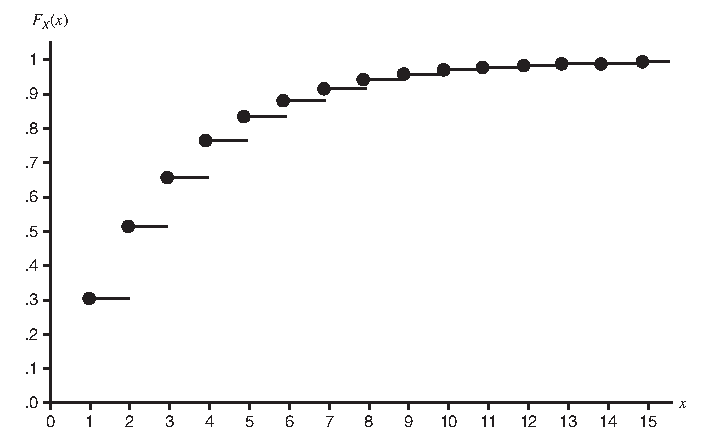
\includegraphics[width=.88\textwidth]{assets/chapter1/fig-1-5-2.pdf}
\caption{几何分布的cdf，$p=.3$}\label{fig:1.5.2}
\end{figure}

\begin{example}[有跳跃的cdf]\label{ex:1.5.6}\index{SI0240@混合}
若$F_X$不是$x$的连续函数，它可以由连续片段与跳跃混合而成.例如，对某个满足$1>\varepsilon>0$的$\varepsilon$，将\eqref{eq:1.5.5}中的$F_X(x)$修改为
\begin{equation}\label{eq:1.5.6}
F_Y(y)=\begin{cases}
\dfrac{1-\varepsilon}{1+e^{-y}},&y<0,\\[5pt]
\varepsilon+\dfrac{1-\varepsilon}{1+e^{-y}},&y\ge0,
\end{cases}
\end{equation}
则$F_Y(y)$是某个随机变量$Y$的cdf（见习题\ref{exercise:1.47}）.函数$F_Y$在$y=0$处有高度为$\varepsilon$的跳跃，其余地方都连续.若观察某个仪表的读数，而该读数理论上可处于$-\infty$与$\infty$之间的任何位置，则这个模型可能合适.不过，这台仪表有时会卡在0处.于是可以用$F_Y$对观测建模，其中$\varepsilon$为仪表卡住的概率.
\end{example}

cdf是连续还是有跳跃，对应于相关随机变量是否连续.事实上，根据这种对应关系来定义连续随机变量很方便.
\begin{definition}\label{def:1.5.7}\index{SI0867@连续}\index{SI0868@离散}
若$F_X(x)$是$x$的连续函数，则随机变量$X$称为连续型（continuous）.若$F_X(x)$是$x$的阶梯函数，则随机变量$X$称为离散型（discrete）.
\end{definition}

本节最后给出一个定理，正式说明$F_X$完全确定随机变量$X$的概率分布.这个结论成立的前提是，仅对$\mathscr B^1$中的事件$A$定义$P(X\in A)$；其中$\mathscr B^1$是包含所有形如$(a,b)$、$[a,b)$、$(a,b]$和$[a,b]$的实数区间的最小$\sigma$代数.若对更大的事件类定义概率，则两个随机变量可能具有相同的分布函数，却并非对每个事件都有相同的概率（见\hyperref[bib:source78]{Chung（1974），第27页}）.与大多数统计应用一样，本书只关心区间、区间的可数并或交等事件，因此不考虑这类病态情况.我们首先需要两个随机变量同分布的概念.

\sourcepageanchor{59}

\begin{definition}\label{def:1.5.8}\index{SI0869@同分布}
若对每个集合$A\in\mathscr B^1$都有$P(X\in A)=P(Y\in A)$，则随机变量$X$与$Y$称为同分布（identically distributed）.
\end{definition}
注意，同分布的两个随机变量未必相等.也就是说，定义\ref{def:1.5.8}并不是说$X=Y$.

\begin{example}[同分布的随机变量]\label{ex:1.5.9}
考虑例\ref{ex:1.4.3}中抛一枚公平硬币三次的试验.定义随机变量$X$与$Y$为
\begin{equation*}\begin{aligned}
X&=\text{观察到正面的次数},\\
Y&=\text{观察到反面的次数}.
\end{aligned}\end{equation*}
$X$的分布已在例\ref{ex:1.4.3}中给出，容易验证$Y$的分布与之完全相同.也就是说，对每个$k=0,1,2,3$，都有$P(X=k)=P(Y=k)$.因此$X$与$Y$同分布.然而，没有任何样本点满足$X(s)=Y(s)$.
\end{example}

\begin{theorem}\label{thm:1.5.10}
下列两个陈述等价：
\begin{enumerate}[label=\alph*.]
\item\label{item:1.5.10a}随机变量$X$与$Y$同分布.
\item\label{item:1.5.10b}对每个$x$都有$F_X(x)=F_Y(x)$.
\end{enumerate}
\end{theorem}
\begin{proof}
为证明等价性，必须说明两个陈述相互蕴含.先证明\hyperref[item:1.5.10a]{(a)}$\implies$\hyperref[item:1.5.10b]{(b)}.

因为$X$与$Y$同分布，对任意集合$A\in\mathscr B^1$，有$P(X\in A)=P(Y\in A)$.特别地，对每个$x$，集合$(-\infty,x]$属于$\mathscr B^1$，且
$$F_X(x)=P(X\in(-\infty,x])=P(Y\in(-\infty,x])=F_Y(x).$$
反向的蕴含关系，即\hyperref[item:1.5.10b]{(b)}$\implies$\hyperref[item:1.5.10a]{(a)}，要难证得多.上面的论证说明，若$X$与$Y$的概率在所有集合上相同，则它们在区间上也相同.现在必须证明相反方向，即若$X$与$Y$的概率在所有区间上相同，则它们在所有集合上都相同.证明这一点需要大量使用\index{SI0974@生成的}\semanticindexanchor{974:59}$\sigma$代数，这里不展开细节.只需指出，只要证明两个概率函数在所有区间上一致就够了（\hyperref[bib:source78]{Chung，1974，第2.2节}）.
\end{proof}
